\newpage % Rozdziały zaczynamy od nowej strony.
\cleardoublepage % Zaczynamy od nieparzystej strony
\pagestyle{headings}

\section{Implementacja}

\subsection{Budowa systemu}

\subsubsection{Schemat blokowy systemu}

System składa się z dwóch głównych części (Rys. \ref{schemat_blokowy}):
\begin{itemize}
  \item aplikacja wykorzystująca pakiet keras, uruchamiana na komputerze PC
  \item częśc uruchamiana na płytce Z-Turn Board
\end{itemize}

\begin{figure}[h]
  \centering
  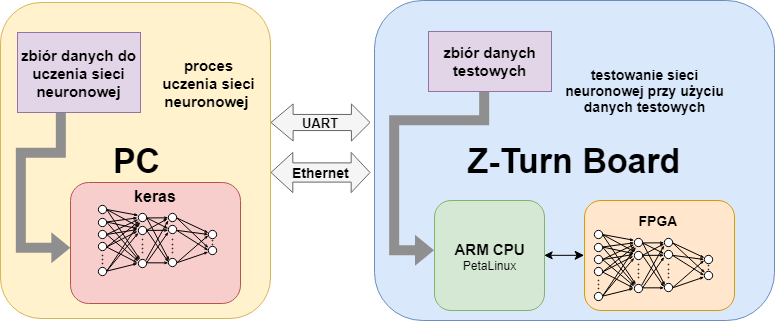
\includegraphics[width=0.8\textwidth]{img/schemat_blokowy.png}
  \caption{Schemat blokowy systemu}
  \label{schemat_blokowy}
\end{figure}

\subsection{Wybór i narzędzi}

Użycie w pracy płytki z układem Zynq determinuje użycie narzędzi wspieranych 
przez firmę Xilinx. Zdecydowano się na użycie najnowszej (w momencie rozpoczęcia 
projektu) wersji oprogramowania 2019.2. Producent zaleca\cite{VivadoGuide} instalację 
programu Vivado na jednym z wspieranych systemów operacyjnych:

\begin{itemize}
  \item Microsoft Windows 7 SP1 Professional (64-bit), English/Japanese 
  \item Microsoft Windows 10.0 1809 Update; 10.0 1903 Update (64-bit), English/Japanese
  \item Red Hat Enterprise Workstation/Server 7.4, 7.5, and 7.6 (64-bit)
  \item SUSE Linux Enterprise 12.4 (64-bit)
  \item CentOS 7.4, 7.5, and 7.6 (64-bit)
  \item Ubuntu Linux 16.04.5 LTS; 16.04.6 LTS; 18.04.1 LTS; 18.04.02 LTS (64-bit)
  \item Amazon Linux 2 LTS (64-bit).
\end{itemize}

\bigskip
W projekcie wykorzystywane było również narzędzie Petalinux, które wymaga 
zainstalowania na maszynie z systemem operacyjnym Linux. Zgodnie z 
dokumentacją\cite{PetalinuxGuide} jest to jedna z trzech dystrybucji:

\begin{itemize}
\item Red Hat Enterprise Workstation/Server 7.4, 7.5, 7.6 (64-bit)
\item CentOS Workstation/Server 7.4, 7.5, 7.6 (64-bit)
\item Ubuntu Linux Workstation/Server 16.04.5, 16.04.6, 18.04.1,18.04.02 (64-bit)
\end{itemize}

\bigskip
Aby zapewnić poprawne działanie narzędzi oraz z racji na sporą popularność i duże 
wsparcie społeczności wybrano dystrybucję Ubuntu 18.04.02 LTS. Przy instalacji 
Petalinuxa warto również zwrócić uwagę, że zalecane jest aż 100GB wolnego miejsca 
na dysku twardym. 

\subsection{Projekt systemu w środowisku Vivado}

Zdecydowano się na zastosowanie blokówpamięci BRAM do komunikacji pomiędzy 
blokiem IP implementowanym z użyciem HLS, a procesorem. Zrzut ekranu przedstawiający 
schemat systemu w środowisku Vivado umieszczono na Rys. \ref{vivado-block-design}

\begin{figure}
  \centering
  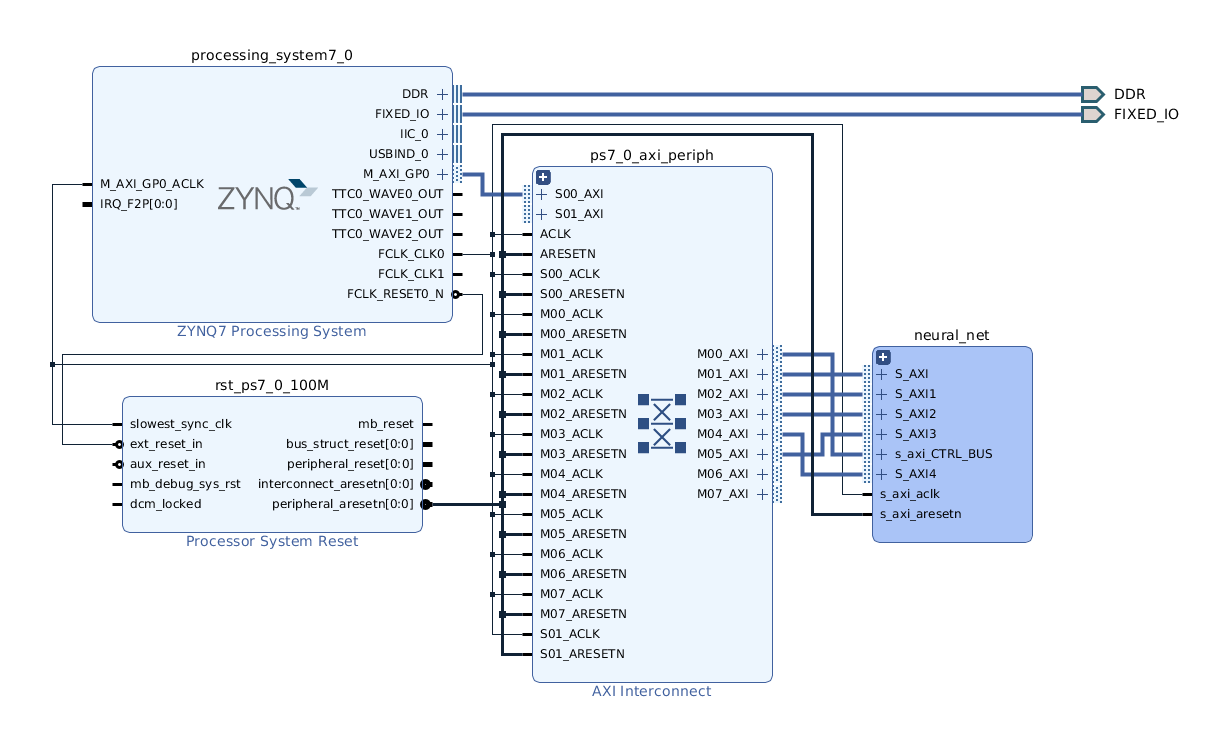
\includegraphics[width=0.8\textwidth]{img/vivado-block-design.png}
  \caption{Schemat systemu przedstawiony w narzędziu Vivado}
  \label{vivado-block-design}
\end{figure}


\subsection{Wykorzystanie metody HLS}
Przy użyciu metody HLS możliwe jest stworzenie własnego bloku IP (ang. 
Intellectual Property), który następnie jest umieszczany w katalogu IP i można 
go wielokrotnie wykorzystać w projekcie RTL (ang. Register Transfer Level).
Do projektu z użyciem HLS (Rys.\ref{hls_design_flow}) potrzebny jest plik 
z algorytmem w języku C/C++ lub System C, plik testowy napisany w języku C 
(ang. test bench) oraz plik z opisem ograniczeń sprzętowych (ang. constraints).
Kolejne etapy projektu z wykorzystaniem metody HLS \cite{hlsXilinxGuide}:

\begin{enumerate}
    \item Kompilacja, wykonanie (symulacja) i debugowanie algorytmu napisanego w języku C
    \item Synteza algorytmu w języku C w implementację RTL
    \item Wygenerowanie raportu i analiza projektu
    \item Zweryfikowanie implementacji RTL
    \item Spakowanie implementacji RTL w blok IP
\end{enumerate}


\begin{figure}
  \centering
  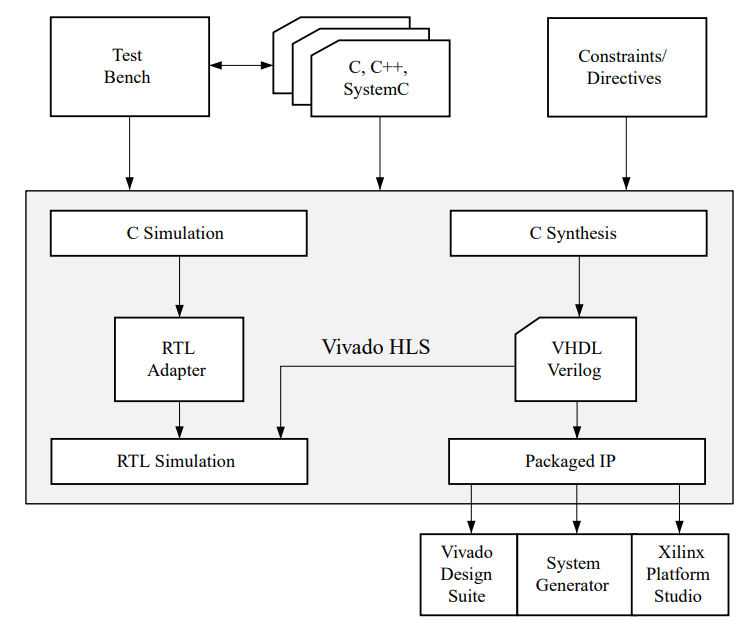
\includegraphics[width=0.8\textwidth]{img/hls_design_flow.png}
  \caption{Proces projektowania przy użyciu metody HLS}
  \label{hls_design_flow}
\end{figure}

Zastosowanie syntezy wysokiego poziomu umożliwia przeniesienie algorytmu 
napisanego w języku C/C++ lub System C na implementację w układzie FPGA. 
Dodatkową zaletą metody HLS jest dostępność bibliotek do przetwarzania 
obrazów oraz ułatwiających implementację operacji matematycznych. 

Przy tworzeniu nowego projektu w Vivado HLS (Rys. \ref{hls_new_project}) trzeba podać 
urządzenie na którym uruchamiany będzie blok IP. Jeśli płytka nie jest widoczna na 
liście należy dodać pliki opisujące ją w odpowiednim katalogu, gdzie zostało 
zainstalowane narzędzie Vivado HLS.  

\begin{figure}
  \centering
  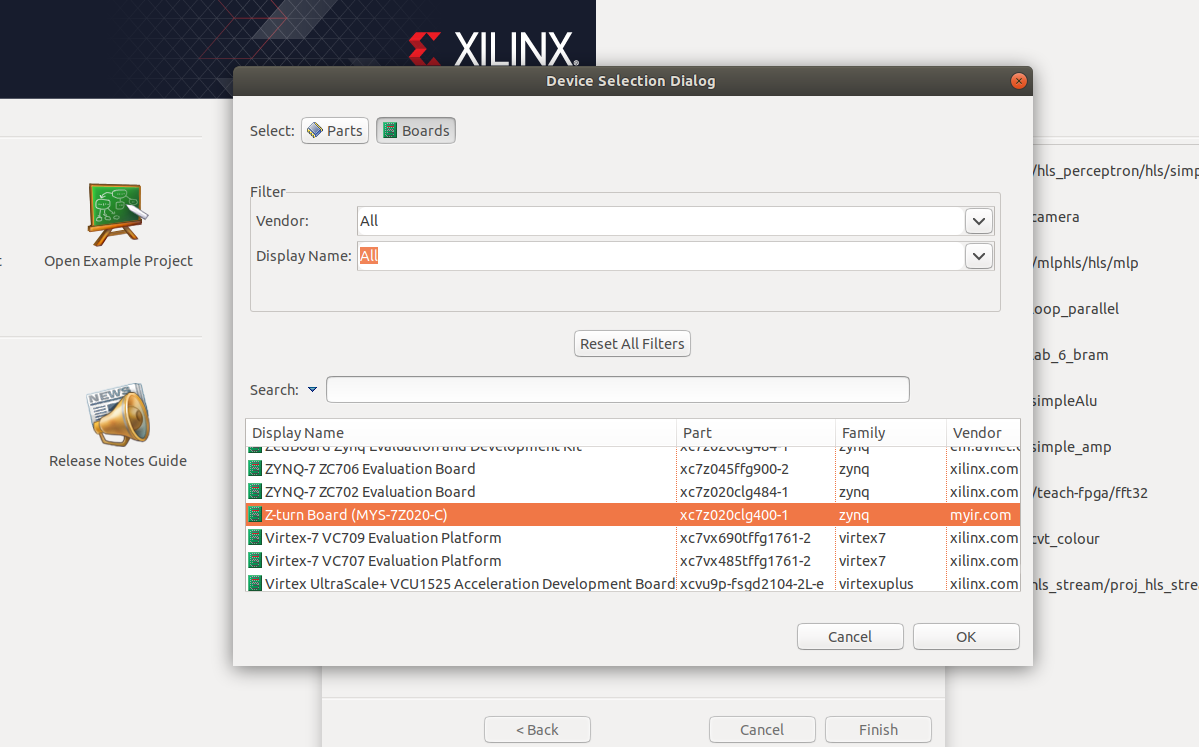
\includegraphics[width=0.8\textwidth]{img/vivado-hls-new.png}
  \caption{Wybór płytki podczas tworzenia projektu w Vivado HLS}
  \label{hls_new_project}
\end{figure}


\subsection{Petalinux}

\subsection{Uczenie Sztucznej Sieci Neuronowej}

\subsection{Zbiór danych wejściowych}

W procesie uczenia oraz testowania poprawności działania modelu sztucznej 
sieci neuronowej wykorzystano zbiór odręcznie pisanych cyfr MNIST 
(ang. THE MNIST DATABASE of handwritten digits)
\cite{lecun-mnisthandwrittendigit-2010}


\subsection{Opracowanie modelu ANN}

Przy projektowaniu algorytmu ANN bardzo ważnym aspektem jest odpowiednie dopasowanie 
modelu do danych wejściowych. Najczęściej odbywa się to poprzez wielokrotne testowanie
systemu dla różnych parametrów sieci. W tej pracy początkowym wyborem była architektura
MLP. Przy użyciu pakietu \emph{keras} zaimplementowano model zawierający 3 warstwy:

\begin{itemize}
  \item warstwę wejściową (784 neuronów)
  \item warstwę ukrytą (16 neuronów)
  \item warstwę wyjściową (10 neuronów).
\end{itemize}

% Dla dłuższych numerów linii
% potrzebne jest większe wcięcie.
\begin{addmargin}[10mm]{0mm}
  \begin{lstlisting}[
      language=Python,
      numbers=left,
      firstnumber=55,
      caption={Implementacja modelu ANN MLP z jedną warstwą ukrytą},
      aboveskip=0pt
  ]
model = Sequential()
model.add(Flatten())
model.add(Dense(16, use_bias=True, activation='sigmoid'))
model.add(Dense(num_classes, use_bias=True, activation='sigmoid'))

  \end{lstlisting}
  \end{addmargin}

Podczas testowania modelu użyto zbioru MNIST, który zaimportowano wykorzystując
funkcją z pakietu keras. Dokonano uczenia sieci neuronowej przy użyciu zbioru 60000 
obrazów i testowania modelu, podając na wejście sieci 10000 obrazów. Osiągnięto 
dokładność na poziomie 93,6\%. 
Zmiany w postaci dodawania większej ilości nauronów w warstwie ukrytej nie powodowały 
zwiększenia dokładności, więc podjęto decyzję o wykorzystaniu tego modelu w dalszej 
części projektu.

Test loss: 0.22611969929933548\\
Test accuracy: 0.9355999827384949


\subsubsection{Implementacja modelu przy użyciu narzędzia Vivado HLS}

Korzystając z narzędzia Vivado HLS napisano program w języku C++ implementujący 
zaprojektowany wcześniej model sieci. W procesie uczenia ustalono wartości wag i 
biasów. Dwa główne pliki projektu w narzędziu Vivado HLS to core.cpp, zawierający 
implementację algorytmu ANN oraz test\_core.cpp, który służy do przetestowania
algorytmu po przeprowadzeniu syntezy (ang. test bench).   
Pliki zawierające wartości wejściowe, a także wagi i biasy są importowane 
do programu test\_core.cpp. 

Pierwszym etapem jest Symulacja C, która jest wstępną weryfikacją poprawności
algorytmu. Do przeprowadzenia symulacji wykorzystano dane wyeksportowane przy użyciu 
skryptu \emph{keras2fpga.py} i zapisane w plikach hls\_biases.h, hls\_weights.h oraz 
hls\_input.h. Wynikiem symulacji jest plik .log, w którym można znaleźć informacje o
tym jak przebigało wywołanie testowanych funkcji.\ref{hls_design_sim}

\begin{figure}
  \centering
  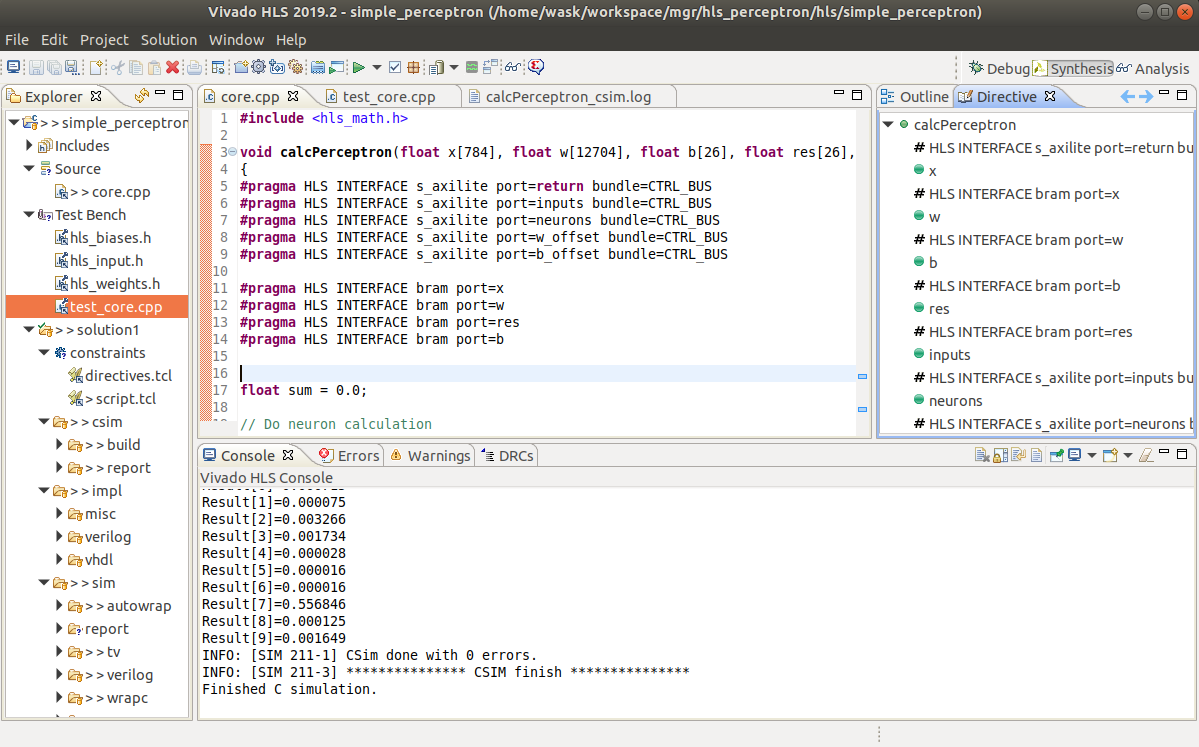
\includegraphics[width=0.8\textwidth]{img/vivado_hls_sim.png}
  \caption{Wynik poprawnie przeprowadzonej symulacji w Vivado HLS}
  \label{hls_design_sim}
\end{figure}


Następnie wykonywana jest synteza oraz kosymulacja, umożliwiająca 
weryfikację poprawności syntezy. Ponadto narzędzie generuje raport, który przedstawia
informacje na temat zużycia zasobów i opóźnień czasowych. Po prawidłowym 
przeprowadzeniu kosymulacji należy użyć opcji \emph{Export RTL}, co umożliwia 
dodanie nowego bloku IP do projektu w narzędziu Vivado. 



\subsection{Testowanie systemu}

% Algorytmy rozpoznawania obiektów mogą być wywoływane na różne sposoby. 
% Jedną z metod jest rejestrowanie obrazu z możliwie maksymalną ilością klatek 
% na sekundę, analizowanie każdej ramki, wyszukiwanie obiektów i klasyfikacja za 
% pomocą algorytmu ANN. Drugim, prostszym w implementacji sposobem, jest wywoływanie 
% zarejestrowania obrazu w momencie, gdy użytkownik, chce dokonać klasyfikacji 
% obiektu, który znajduje się w zasięgu obiektywu kamery, a na zarejestrowanym 
% obrazie nie ma innych obiektów. Z powodu ograniczeń zasobów systemu, na którym 
% aplikacja była testowana oraz ograniczonego czasu wykonania projektu, podjęto 
% decyzję o zastosowaniu drugiej metody. 


